% !TeX root = Tesis.tex
% !TeX encoding = UTF-8
% !TeX spellcheck = es_ES
\chapter{Chapter 2}
\label{cap3}
\onehalfspacing


\section{The N + GB + EA diagram}\label{sec:ngbad}

Nuestro punto de partida es el diagrama de los datos de expresión genética del análisis de componentes principales para la materia blanca del cerebro, mostrado en la Fig. \ref{fig:fig1a}. Como se puede notar en la figura, las dos primeras componentes principales capturan más del 80 \% de la varianza del sistema. Por lo tanto, es una representación bidimensional adecuada de la distribución real de los puntos en el espacio de expresión genética.

\begin{figure}[!ht]
	%TODO: rehacer la figura para cambiar el label AD por EA
	\centering
	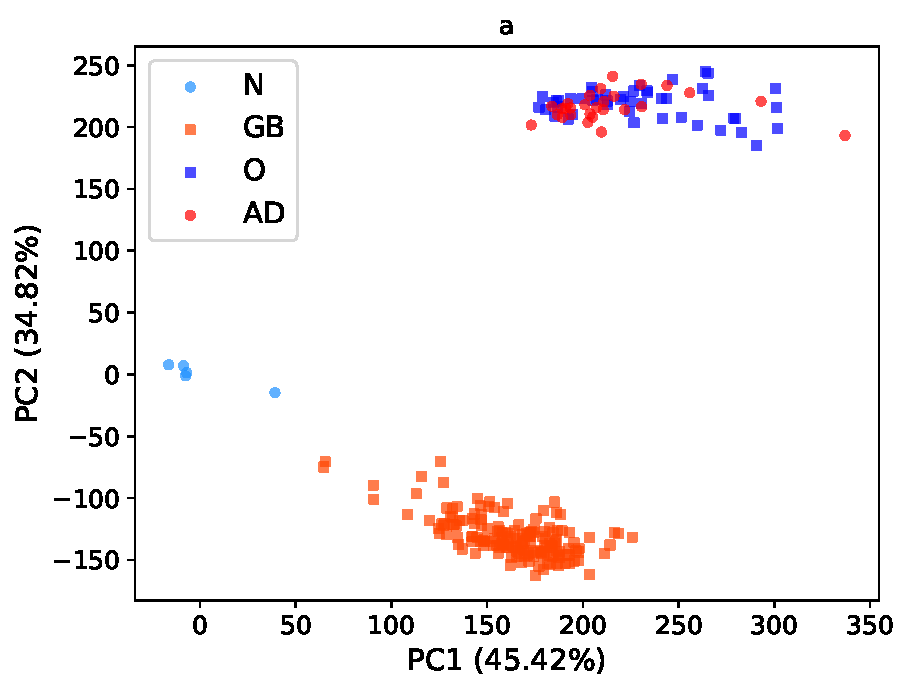
\includegraphics{figures/Fig_1a.pdf}
	\caption{\label{fig:fig1a}
		Análisis de componentes principales para los datos de expresión genética.}
\end{figure}

En la figura se pueden apreciar 4 grupos de muestras. Las muestras marcadas como N y GB corresponden, a especímenes patológicamente normales y tumorales en los datos del Atlas del Genoma del Cáncer (TCGA, \href{https://www.cancer.gov/tcga}{https://www.cancer.gov/tcga}) para el Glioblastoma \cite{Brennan_2013}. Estas son tomadas durante procedimientos quirúrgicos. Los tumores se pueden localizar en diferente zonas cerebrales pero, como es común en el Glioblastoma, estos son tumores tomados de la sustancia blanca del cerebro \cite{ellingson2013probabilistic}. Los centros de las nubes de muestras de N y GB en el espacio de expresión genética definen, respectivamente, los atractores Normal (homeostático) y Glioblastoma de Kauffman \cite{Huang_2009, Gonzalez_2023}. De hecho, la acumulación de puntos en una determinada región de este espacio indica que esta es un atractor de la Red de regulación Genética que gobierna la dinámica del sistema.

Hay 5 muestras N de pacientes con edades en el rango entre 49 y 74 años, mientras que el intervalo de edades de las 169 muestras de GB es entre 21 y 89 años. Las pacientes femeninas representan aproximadamente dos tercios de la cohorte.

Por otro lado, los grupos etiquetados como EA y O corresponden a las muestras de la materia blanca del cerebro de la enfermedad del Alzheimer y del grupo de control (\textit{old}) en el estudio longitudinal del Instituto Allen sobre envejecimiento y la demencia (\href{https://aging.brain-map.org/}{https://aging.brain-map.org/}) \cite{Miller_2017}. Las muestras son tomadas \textit{post mortem}. El grupo O está conformado por 47 muestras, mientras que en el grupo EA hay 28. El intervalo de edad para todas estas muestras es entre 77 y 101 años. El diagnóstico de la EA está respaldado por pruebas cognitivas y otras pruebas clínicas. Alrededor del 40 \% de la cohorte son mujeres.

La Fig. \ref{fig:pcaotoad} es una reconstrucción de la figura 3 de la referencia \cite{Gonzalez_2021}. En esta se muestra los resultados del PCA para los datos de expresión genética de la materia blanca del cerebro del Instituto Allen. La primera componente principal (PC1), la cual contiene el $24.7 \%$ de la varianza total, discrimina entre las muestra de O y EA. La posición del centro de la nube de O en este eje es $\left\langle x_1 \right\rangle  = 0 $, y para la EA es $\left\langle x_1 \right\rangle = 40.97 $. Sin embargo, los radios de las nubes de las muestras de O y EA son más grandes que la distancia entre los centros, que son $80.69$ y $72.64$ respectivamente.
%\alert{Estudiamos la transición de O hacia EA en la referencia \cite{Gonzalez_2021}}. En la Fig. \ref{fig:otoad}

\begin{figure}[!htb]
	%TODO: replot this figure
	%TODO: cambiar el label ND por O y AD por EA
	\centering
	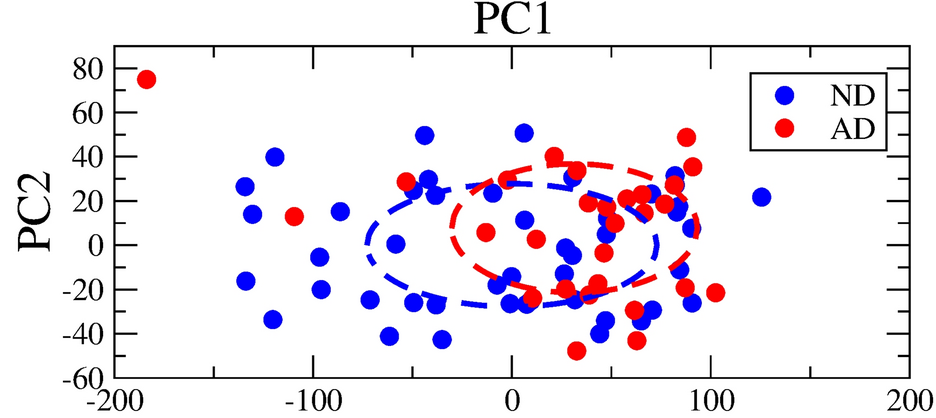
\includegraphics[width=0.75\linewidth]{figures/pca_o_to_ad_1.png}
	\caption{Figura tomada de la referencia \cite{Gonzalez_2021}.}
	\label{fig:pcaotoad}
\end{figure}

Es bien conocido el papel de la edad en la EA, especialmente en ancianos \cite{alz2019}. Por lo tanto, podemos usar la edad como una variable de tiempo para seguir la transición. A pesar del número relativamente pequeño de muestras, se realizó un análisis de regresión lineal de la posición media de $\left\langle x_1 \right\rangle$ en función de la edad en las muestras de O, Fig. \ref{fig:otoad}a, muestra que $\left\langle x_1 \right\rangle = -287.12 + 3.24 \cdot edad$. En las muestras de la EA, sin embargo, no se encontró correlación entre $\left\langle x_1 \right\rangle$ y la edad observada. Por lo tanto, la posición de la zona EA es aproximadamente fija, y la nube de muestras de O muestra una deriva hacia el mínimo de EA a medida que aumenta la edad.

\begin{figure}[!htb]
	%TODO: replot this figure
	\centering
	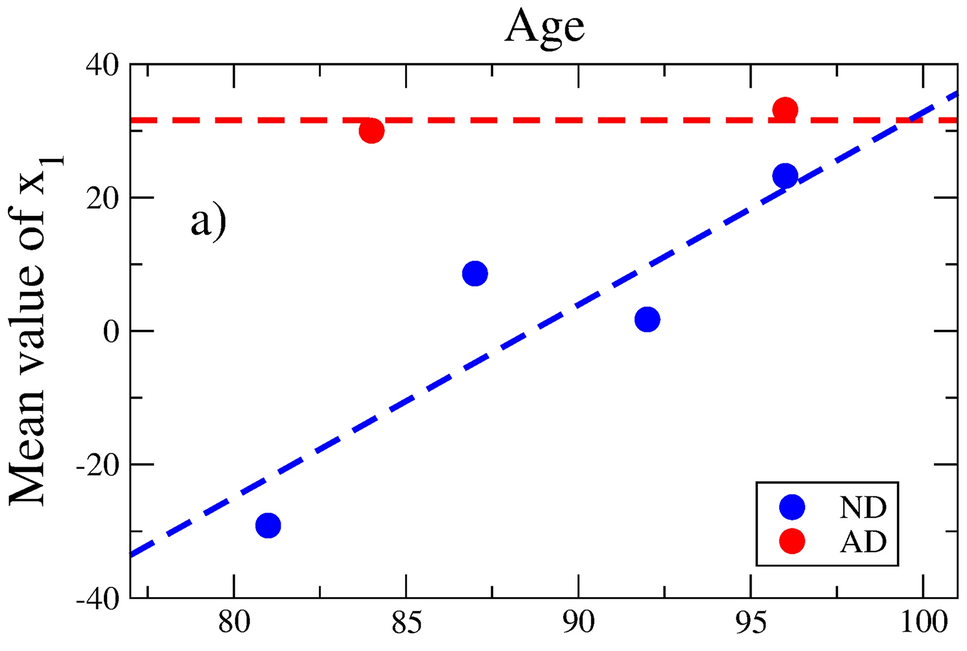
\includegraphics[width=0.7\linewidth]{figures/O_to_AD_1.png}
	\caption{Figura tomada de la referencia \cite{Gonzalez_2021}}
	\label{fig:otoad}
\end{figure}

Una mejor ilustración de este hecho viene representada en la Fig. \ref{fig:supplotoad}, donde se compara la densidad de probabilidad de las muestras de O y de la EA. Se definen cuatro intervalos de edades, que contienen aproximadamente la misma cantidad de muestras de O: [77, 84], [84, 90], [90, 95], [95, 100+]. La probabilidad total de las muestras de la EA es mostrada en los cuatro paneles. Es aparente un desplazamiento de las muestras de O hacia la zona de la EA.


\begin{figure}[!htb]
	%TODO: hacer un replot de la figura
	\centering
	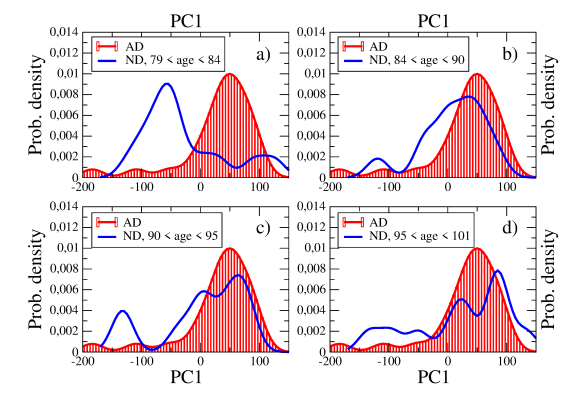
\includegraphics[width=0.75\linewidth]{figures/suppl_otoad.png}
	\caption{Densidad de probabilidad de las muestras de O y de la EA a lo largo del eje de PC1. Cada panel es para un intervalo de edad para las muestras de O. La probabilidad de la EA, la cual es aproximadamente independiente de la edad, es mostrada en los cuatro paneles. Figura tomada de la referencia \cite{Gonzalez_2021}}
	\label{fig:supplotoad}
\end{figure}

Esta propiedad sugiere que el centro de la nube de muestras de la EA define un atractor en el espacio de expresión genética. Las muestras de O parecen ser atrapadas por el atractor de la EA en el proceso del envejecimiento.